\section{Adaptive Recommenders}
\label{sec:usermetamodeling}

\emph{Adaptive Recommenders} (AR) is our technique for combining many recommender systems
in a way that is optimal for the each user and item.
Given that we wish to predict the relevance of an item to a user,
using many methods that consider disjoint data patterns,
there are two important questions:

\begin{enumerate*}
  \item What rating does each method predict?
  \item How accurate will each of these predictions be?
\end{enumerate*}

Recommender systems traditionally only care about the first question.
A single method is used to predict an unknown rating.
Modern aggregation techniques goes one step further, and combines many methods using a generic (often weighted) combination.
We wish to make the aggregation \emph{adaptive},
so that the aggregation itself depends on which user and which item we are considering.

Formally, we define adaptive recommenders as \emph{adapting a set of recommender systems
with another complementary set of recommender systems} 
(see Figure \ref{fig:adaptiveusermodeling}).
This then is a form of meta-modeling, where one set of modeling methods is adapted by another set of modeling methods.
The first set creates standard prediction scores, and answers the first question.
The second set predicts how accurate each method will be for the current user and item,
answering the second question.
The interesting bit is that AR can use recommender systems for both these tasks, as we shall see.
A system for adaptive recommenders is specified by a 6-tuple:

\begin{eqnarray*}
  \mathrm{AR} &=& (Items, Users, Ratings, Framework, Methods, Adapters)\\
              &=& (I,U,R,F,M,A).
\end{eqnarray*}
%
We have sets of $Users$ and $Items$, and a set of $Ratings$.
Any user $u \in U$ can produce a rating $r \in R$ of an item $i \in I$.
As mentioned, items can be just about anything, for example documents, websites, movies, events, or indeed, other users.
The ratings can be explicitly provided by users, for example by rating movies,
or they can be implicitly extracted from existing data, for example by mining query logs.

We use the term \emph{rating} loosely --- equivalent terms include \emph{relevance}, \emph{utility},
\emph{score} or \emph{connection strength}. In other words, this is a measure of what a user thinks of an item
in the current domain language. However, since \emph{rating} will match the case study we present in the next chapter,
we will be using this term. 

\begin{figure}[t]
  \centering 
  \begin{minipage}{0.49\textwidth}
    \centering 

    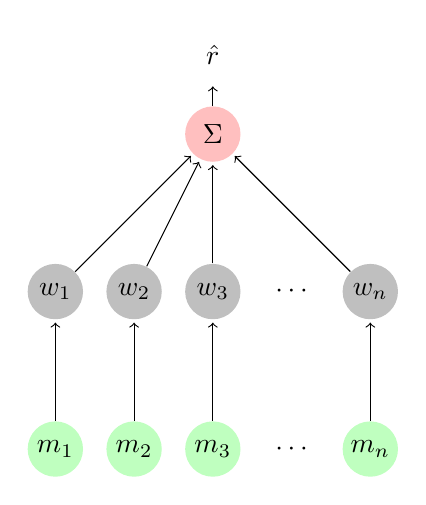
\begin{tikzpicture}[shorten >=1pt,->,draw=black, node distance=\layersep]
      \tikzstyle{every pin edge}=[<-,shorten <=2pt]
      \tikzstyle{node}=[circle,fill=black!25,minimum size=20pt,inner sep=0pt];
      \tikzstyle{method}=[node,fill=green!25];
      \tikzstyle{weight}=[node,fill=black!25];
      \tikzstyle{error}=[node,fill=blue!25];
      \tikzstyle{agg}=[node,fill=red!25];
      \tikzstyle{txt}=[node,fill=white];
       
      \node[method] (M1) at (0,-6) {$m_1$};      
      \node[method] (M2) at (1,-6) {$m_2$};         
      \node[method] (M3) at (2,-6) {$m_3$};         
      \node[txt]    (MS) at (3,-6) {$\cdots$}; 
      \node[method] (MN) at (4,-6) {$m_n$};
      \node[weight] (W1) at (0,-4) {$w_1$};      
      \node[weight] (W2) at (1,-4) {$w_2$};         
      \node[weight] (W3) at (2,-4) {$w_3$};         
      \node[txt]    (WS) at (3,-4) {$\cdots$}; 
      \node[weight] (WN) at (4,-4) {$w_n$};
      \node[agg]    (AG) at (2,-2) {$\Sigma$};
      \node[txt]    (RS) at (2,-1)  {$\hat{r}$};
      
      \path (M1) edge (W1);
      \path (M2) edge (W2);
      \path (M3) edge (W3);
      \path (MN) edge (WN);
      \path (W1) edge (AG);
      \path (W2) edge (AG);
      \path (W3) edge (AG);
      \path (WN) edge (AG);
      \path (AG) edge (RS);
    \end{tikzpicture}
  \end{minipage} 
  \hfill 
  \begin{minipage}{0.49\textwidth}
    \centering 

    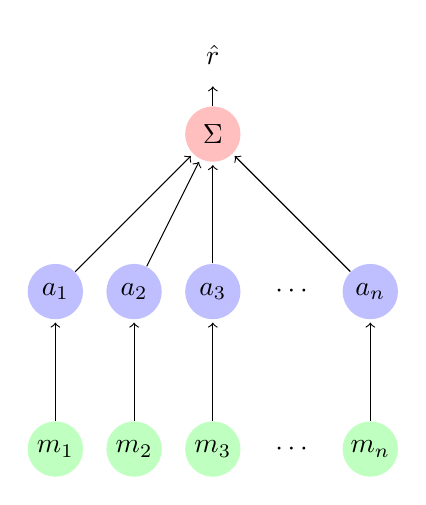
\begin{tikzpicture}[shorten >=1pt,->,draw=black, node distance=\layersep]
      \tikzstyle{every pin edge}=[<-,shorten <=2pt]
      \tikzstyle{node}=[circle,fill=black!25,minimum size=20pt,inner sep=0pt];
      \tikzstyle{method}=[node,fill=green!25];
      \tikzstyle{weight}=[node,fill=black!25];
      \tikzstyle{error}=[node,fill=blue!25];
      \tikzstyle{agg}=[node,fill=red!25];
      \tikzstyle{txt}=[node,fill=white];
       
      \node[method] (M1) at (0,-6) {$m_1$};      
      \node[method] (M2) at (1,-6) {$m_2$};         
      \node[method] (M3) at (2,-6) {$m_3$};         
      \node[txt]    (MS) at (3,-6) {$\cdots$}; 
      \node[method] (MN) at (4,-6) {$m_n$};
      \node[error]  (E1) at (0,-4) {$a_1$};      
      \node[error]  (E2) at (1,-4) {$a_2$};         
      \node[error]  (E3) at (2,-4) {$a_3$};         
      \node[txt]    (ES) at (3,-4) {$\cdots$}; 
      \node[error]  (EN) at (4,-4) {$a_n$};
      \node[agg]    (AG) at (2,-2) {$\Sigma$};
      \node[txt]    (RS) at (2,-1)  {$\hat{r}$};
      
      \path (M1) edge (E1);
      \path (M2) edge (E2);
      \path (M3) edge (E3);
      \path (MN) edge (EN);
      \path (E1) edge (AG);
      \path (E2) edge (AG);
      \path (E3) edge (AG);
      \path (EN) edge (AG);
      \path (AG) edge (RS);
    \end{tikzpicture}
  \end{minipage} 
  \vspace{2em}
  \caption[Comparison of Aggregation and Adaption]{
    Comparison of aggregation and adaption:
    (left) modern aggregation approaches uses a set of pretrained weights
    to prioritize each modeling method.
    The weighted predictions are aggregated into a final prediction $\hat{r}$.
    (right) Adaptive user modeling employs secondary modeling methods instead
    of weights. These estimate the accuracy of the initial method
    for the current user and item.
  }
  \label{fig:layer:comparison}
\end{figure}




The $Framework$ variable specifies how the data is represented.
The two canonical ways of representing users, items and ratings are graphs and matrices (see Section \ref{sec:recommender}).
We shall use a matrix, where the first dimension corresponds to users, the second to items, and each populated cell is an explicit or implicit rating:

\begin{eqsp}
 R_{u,i} =
 \begin{pmatrix}
  r_{1,1} & r_{1,2} & \cdots & r_{1,i} \\
  r_{2,1} & r_{2,2} & \cdots & r_{2,i} \\
  \vdots  & \vdots  & \ddots & \vdots  \\
  r_{u,1} & r_{u,2} & \cdots & r_{u,i}
 \end{pmatrix}.
\end{eqsp}
%
As we wish to leverage disjoint data patterns, we have a set of modeling $Methods$, 
with their own ways of estimating unknown ratings. 
Each model $m \in M$ is used to compute independent and hopefully complimentary predictions.
In our case, these methods are recommender systems.

As demonstrated in Chapter \ref{chap:theory}, there are many different recommendation algorithms,
that consider different aspects in the data, for example users, items and ratings, as well as 
sources such as intra-user connections in social networks or intra-item connections in information retrieval systems.
Examples of such recommender systems include Slope One predictions, SVD factorization and Nearest Neighbor weighted predictions
(see Section \ref{subsec:recommender:examples}).
These methods predict unknown connections between users and items based on some pattern in the data,
for example user profile similarity, rating correlations or social connections.
As previously explained, to achieve the best possible combined result, we wish to use methods that look at disjoint patterns, 
i.e. complementary predictive parts of the data (see Section \ref{sec:aggregate}).

The $Adapters$ part of our 6-tuple refers to the second level of recommender systems.
In traditional prediction aggregation this is a simple linear function for combining the different predictions,
for example by pre-computing a set of weights, one per method.
As found by \citet[p6]{Bell2007} the accuracy of the combined predictor is more dependent on the 
ability of the various predictors to expose different aspects of the data, than on 
the individual accuracy of the predictors.
As described in Section \ref{sec:aggregate}, multiple prediction results are normally 
combined into a final singular result,
based on a generalized combination found by minimizing some error across all users.

With adaptive recommenders, the $Adapters$ are themselves recommender systems 
(see Figure \ref{fig:layer:comparison}).
However, instead of modeling users, we wish to model the behavior of the recommender systems.
More specifically, we wish to model the \emph{accuracy} of our recommender systems.
Methods in this second layer are used to predict how accurate each of their corresponding basic recommenders will be.
It is these methods that will allow us to do adaptive aggregation based on the current user and item.
We then have two distinct layers of recommender systems 
(see Figure \ref{fig:adaptiveusermodeling}):

\begin{figure}
  \center
  \def\layersep{1.8cm}
  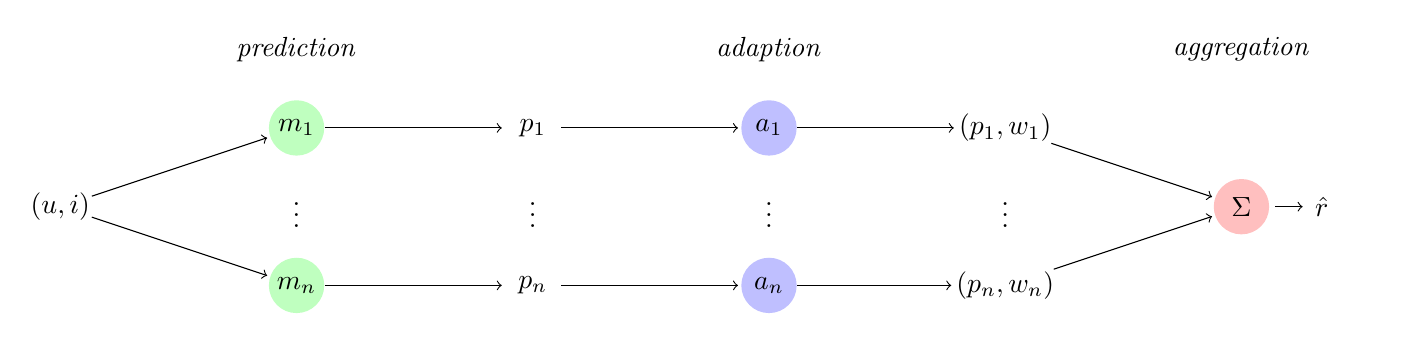
\begin{tikzpicture}[shorten >=1pt,->,draw=black, node distance=\layersep]

    \tikzstyle{every pin edge}=[<-,shorten <=2pt]
    \tikzstyle{node}=[circle,fill=black!25,minimum size=20pt,inner sep=0pt]
    \tikzstyle{input node}=[node, fill=green!25];
    \tikzstyle{output node}=[node, fill=red!25];
    \tikzstyle{hidden node}=[node, fill=blue!25];
    \tikzstyle{annot} = [text width=10em, text centered]
    \tikzstyle{txt}=[node,fill=white];
    
    \node[txt] (UI) at (0,-2) {$(u,i)$};  

    \node[input node] (I-1) at (\layersep,-1) {$m_1$};
    \node[txt]        (I-D) at (\layersep,-2) {$\vdots$};
    \node[input node] (I-N) at (\layersep,-3) {$m_n$};
    
    \node[txt] (P-1) at (\layersep*2, -1) {$p_1$};
    \node[txt] (P-D) at (\layersep*2, -2) {$\vdots$};
    \node[txt] (P-N) at (\layersep*2, -3) {$p_n$};

    \node[hidden node] (H-1) at (\layersep*3, -1) {$a_1$};    
    \node[txt]         (H-D) at (\layersep*3, -2) {$\vdots$};    
    \node[hidden node] (H-N) at (\layersep*3, -3) {$a_n$};    

    \node[txt] (R-1) at (\layersep*4, -1) {$(p_1,w_1)$};
    \node[txt] (R-D) at (\layersep*4, -2) {$\vdots$};
    \node[txt] (R-N) at (\layersep*4, -3) {$(p_n,w_n)$};
    
    % hidden helper node
    \node[txt] (HH)  at (\layersep*5,-1) {};

    % Draw the output layer node
    \node[output node,pin={[pin edge={->}]right:$\hat{r}$}] at (\layersep*5,-2) (O) {$\Sigma$};
    
    \path (UI) edge (I-1);
    \path (UI) edge (I-N);

    \path (I-1) edge (P-1);
    \path (I-N) edge (P-N);

    \path (P-1) edge (H-1);
    \path (P-N) edge (H-N);

    \path (H-1) edge (R-1);
    \path (H-N) edge (R-N);

    \path (R-1) edge (O);
    \path (R-N) edge (O);

    % Annotate the layers
    \node[annot,above of=I-1, node distance=1cm] {\emph{prediction}};
    \node[annot,above of=H-1, node distance=1cm] {\emph{adaption}};
    \node[annot,above of=HH,  node distance=1cm] {\emph{aggregation}};
  \end{tikzpicture}

  \vspace{1em}
  \caption[The Layers of Recommenders]{
    Layers of recommenders. 
  }
  \label{fig:adaptiveusermodeling}
\end{figure}


\begin{enumerate}
  \item
    \emph{The methods layer} consists of traditional recommender systems, that use a single aspect of the data to produce predictions.
    When presented with an item and a user, these methods produce a predicted rating $\hat{r}_{u,i}$ based on their algorithms.
  \item
    \emph{The adaptive layer} is another set of corresponding recommenders that work a bit differently.
    These methods take an item and a user and estimates how well its underlying method will perform this prediction.
    The accuracy estimations are then combined with the predictions by aggregation.
    However, each of these adaptive methods do not have to employ the same algorithm as their corresponding methods.
\end{enumerate}

Another way of describing (and implementing) the two levels is with
the $\mathrm{map}$ and $\mathrm{reduce}$ functions of functional programming.
We can express prediction aggregation as:

\begin{eqsp}
  \hat{r}_{u,i} = \mathrm{reduce}(u, i, \mathrm{map}(M, u, i)).
\end{eqsp}

First, each modeling method is applied by the $\mathrm{map}$ function, with the current user, item and set of modeling methods as input.
This operation returns a set of scalar prediction values. 
These values are then combined by the $\mathrm{reduce}$ function, which also takes the current user and item as input.
In our terms, $\mathrm{map}$ is the methods layer, and $\mathrm{reduce}$ is the adaptive layer.
If we wish to do rank aggregation, the equation is a bit different:

\begin{eqsp}
  \tau_{u,n} = \mathrm{reduce}(u, \mathrm{map}(M,u,n)).
\end{eqsp}

Here, $\tau_{u}$ is the list of recommended items for user $u$ (following the notation in \citet[p3]{Dwork2001}).
Note that there is no input item in this formula as we wish to produce a ranking of the top $n$ recommended items.
The result is an adaptively sorted list of the top $n$ items for the current user.
A common use case for rank aggregation is personalized search:
an IR algorithm restricts the item space, which is then adapted by recommender systems,
as we shall see.

Expressing ourselves in terms of $\mathrm{map}$ and $\mathrm{reduce}$ is helpful 
as this will guide our implementation.
Note that our terminology is a bit different from the proper MapReduce framework
for parallel computation (as explained in \citet[p75]{Manning2008}).
However, as with the standard key/value approach to MapReduce,
the fact that our tasks can be run in parallel will help
us implement efficient algorithms.


\subsection{Adaptive Aggregation}

To perform adaptive recommender aggregation, we need the $Adapters$ to be actual recommender systems.
Until now we have talked about both prediction aggregation (scores) and rank aggregation (sorted lists).
For now we shall stick to scalar predictions, but will return to rank aggregation in Section \ref{sec:methods:rank}.

The simplest generalized way of prediction aggregation is to take the average of all predictions made
by the different methods (e.g. \citet[p3]{Aslam2001}):

\begin{eqsp}
  \hat{r}_{u,i} = \frac{1}{N} \sum_{m \in M} p(m,u,i).
\end{eqsp}

Here, $\hat{r}_{u,i}$ is the estimated rating from user $u$ to item $i$,
$N$ is the number of methods in $M$, and $p(m,u,i)$ is the predicted rating from method $m$.
To achieve an even more optimal result, 
many aggregators weigh each method differently (e.g. \cite{Claypool1999}):

\begin{eqsp}
  \hat{r}_{u,i} = \sum_{m \in M} w_{m} \times p(m,u,i) 
  \quad \text{where} \quad 0 \leq w_{m} \leq 1, \quad \sum_{m \in M} (w_m) = 1.
\end{eqsp}

In this equation, $w_m$ is the weight applied to modeling method $m$. 
These weights fall in the range $[0,1]$ and sum up to $1$.
As described in \ref{sec:aggregate}, 
these weights can be estimated by different machine learning methods.
However, as discussed in Section \ref{sec:reasoning},
this is still a generalized result, averaged across every user and item.
The system assumes that the best average result is the best result for individual users and items.
This means that, even with method-specific weights, we are still hindered by the latent subjectivity problem.

In order to leverage as many patterns as possible while sidestepping any latent subjectivity,
we need \emph{adaptive weights} that are computed specifically for combinations of users and items.
This is more difficult than simply estimating generalized weights.
If we wish the weights to be combination-specific, then pre-computing weights for each method becomes unfeasible.
We would have to compute a weight for every method for every possible rating.
The adaptive weights also have to be estimated just as the unknown ratings:

\begin{eqsp}
  \hat{r}_{u,i} = \sum_{m \in M} p_{w}(m,u,i) \times p_{r}(m,u,i)
  \quad \text{where} \quad
  \sum_{m \in M} (p_{w}(m,u,i)) = 1.
\end{eqsp}

Here, $p_w(m,u,i)$ is the predicted optimal weight for method $m$ when applied to user $u$ and item $i$.
Adaptive recommenders is one way to estimating these weights, i.e. one way to implement $p_w$.

We wish to use standard recommender systems for predicting optimal adaptive weights.
To do this, we need to create a matrix (or graph)
that stores known values of how accurate some of the rating predictions will be.

The key insight is that \emph{the predicted accuracy of a method is the opposite of its predicted error}.
By modeling the errors of a method through standard recommender systems,
we can in turn predict errors for untested combinations
(see Figure \ref{fig:adaptiveweights}).
If we predict the error of a recommender system for a user and an item,
we have also predicted its accuracy.
To achieve this, we create an \emph{error matrix}:

\begin{figure}[t]
  \center
  \def\layersep{3cm}
  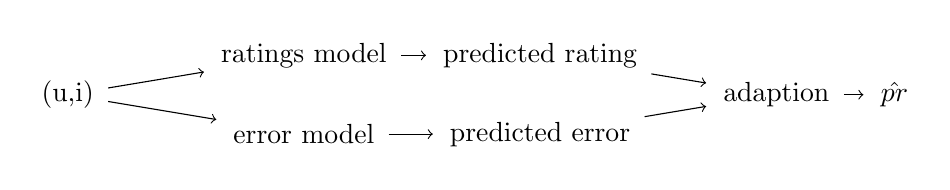
\begin{tikzpicture}[shorten >=1pt,->,draw=black, node distance=\layersep]

    \tikzstyle{every pin edge}=[<-,shorten <=2pt]
    \tikzstyle{rmodel}=[rectangle,fill=green!25,minimum size=20pt,inner sep=5pt]
    \tikzstyle{emodel}=[rectangle,fill=blue!25,minimum size=20pt,inner sep=5pt]
    \tikzstyle{amodel}=[rectangle,fill=red!25,minimum size=20pt,inner sep=5pt]
    \tikzstyle{blank}=[rectangle,fill=white,minimum size=20pt,inner sep=5pt]
    
    \node[blank] (UI) at (0,-0.5) {(u,i)}; 

    \node[blank] (EM) at (\layersep,-1) {error model};
    \node[blank] (RM) at (\layersep,0) {ratings model};
    
    \node[blank] (ER) at (\layersep*2,-1) {predicted error};
    \node[blank] (RR) at (\layersep*2,0) {predicted rating};
 
    \node[blank] (AG) at (\layersep*3,-0.5) {adaption};
    \node[blank] (W) at (\layersep*3.5,-0.5) {$\hat{pr}$}; 
    
    \path (UI) edge (EM);
    \path (UI) edge (RM);
    \path (EM) edge (ER);
    \path (RM) edge (RR);
    \path (ER) edge (AG);
    \path (RR) edge (AG);
    \path (AG) edge (W);
       
  \end{tikzpicture}

  \vspace{1em}
  \caption[Multiple Models for Adaptive Weights]{
    Multiple models for adaptive weights: 
    The data flow through the adaption of a single recommender method.
    The current user and item is fed into two distinct models: the ratings model, which 
    predicts unknown ratings, and the error model, which predicts how accurate 
    this rating will be for the current input. 
    The two predictions are then aggregated into a final part of a rating ($\hat{pr}$).
    Each of the recommender stacks contribute parts to the final rating.
  }
  \label{fig:adaptiveweights}
\end{figure}


\begin{eqsp}
 E_{u,i} =
 \begin{pmatrix}
    e_{1,1} & e_{1,2} & \cdots & e_{1,i} \\
    e_{2,1} & e_{2,2} & \cdots & e_{2,i} \\
    \vdots  & \vdots  & \ddots & \vdots  \\
    e_{u,1} & e_{u,2} & \cdots & e_{u,i}
 \end{pmatrix}
\end{eqsp}

Creating an error matrix for each modeling method is done by splitting the ratings data in two.
The first set can be used for the actual RS modeling, and the second
can be used to populate an error matrix for each RS.

With adaptive recommenders, the standard modeling methods produce error matrices, where some of the cells have values.
A value in this matrix corresponds to the prediction error for a combination of a user and an item.
To achieve this, each modeling method is only trained with a part of the ratings data.
The error matrix is populated from the rest of the data,
by computing the error of every known rating the method was not trained for:

\begin{eqsp}
  \forall (u,i,r) \in (d_e - d_m): E(m)_{u,i} = |r - p(m,u,i)|
  \quad
  \text{where}
  \quad
  d_e,d_m \subset D
\end{eqsp}

Here, $D$ is the current dataset, and
$d_m$ and $d_e$ are subsets of $D$.
$m$ is a modeling method trained with the subset $d_m$.
To populate the error matrix for this method,
we take every rating which have not been used to train the method
and calculate the error of the method on this combination.
Since we are only interested in the magnitude of the error,
we take the absolute value of the measurements.
The result is a sparse error matrix we can use to predict unknown errors.

Notice the similarity of this matrix and the previously introduced ratings matrix.
This similarity is what will allow standard recommender systems
to perform adaptive aggregation.
Whenever we wish to train a new modeling method,
we apply the following algorithm:

\begin{enumerate*}
  \item Split the ratings data into two sets for training and error estimation.
  \item Train the modeling method in its specific way with the first training set.
  \item Use the error estimation data set to create the error matrix.
  \item Train an error model based on the error matrix.
\end{enumerate*}

The error models are trained using standard recommender systems.
After all, the expected input and output is the same.
We have two dimensions, with a sparse set of known connections,
and wish to predict unknown connections from this data.

The result is a set of modeling methods
that can predict the error of a recommender system
when its used on a particular user and item combination.

What will happen when we train a recommender system with the error matrix?
First of all, the errors will be on the same scale as the initial ratings.
Second, just as the ratings matrix will include noise (ratings that
do not contribute to any underlying pattern), this will be 
true for the error matrix as well.

For example, one method might have a large error for a particular user and item combination,
yet still work well for both these elements. 
However, this is just the kind of noise recommender systems are good at pruning away.
What we are interested in are situations where a method
has stable and significant errors for many ratings from a user,
or many ratings of an item.
In this case, there is a pattern where this method does not 
work well for the element in question.
This is exactly the kind of pattern recommender systems are good at identifying.

The same capabilities that makes recommender systems work well
on the ratings matrix, will also make them work well on the error matrix.
The properties we need for predicting ratings
are the same as those needed to predict accuracy.

Of course, some recommender systems will work better than others for the adaptive layer.
Most often we are seeking global patterns in the data.
We are looking for groups of users or items (or both) that suite some 
recommenders especially well, or that some recommenders will not work for.
SVD-based recommenders is one type of RS that can be used for this purpose.
By reducing the method-error space into an \emph{error category space},
we can identify how well a set of groups suite the available methods.
We will get back to this when performing experiments in the next chapter.

When we have an error model for each modeling methods
we can estimate optimal weights.
Whenever we wish to create an adaptive aggregate prediction,
we apply the following algorithm:

\begin{enumerate*}
  \item Collect predictions from the modeling methods for $(u,i)$.
  \item Collect estimated errors for each method for $(u,i)$.
  \item Compute weights for the methods based on their relative predicted errors.
  \item Sum the weighted predictions to get the adaptively predicted rating.
\end{enumerate*}

The next section will explain these steps in detail.
We can now express the prediction phase of adaptive recommenders as an equation.
Each rating/relevance prediction is weighted by its predicted accuracy,
conditioned on the current user and item:

\begin{eqsp}
  \hat{r}_{u,i} = \sum_{(m_{e}, m_{r}) \in M} (1 - 
  \frac{
    p(m_{e},u,i)
  }{
    error(u,i)
  }) \times p(m_{r},u,i)
  \quad
  \text{where}
  \quad
  error(u,i) = \sum_{m_e \in M} p(m_e,u,i) 
\end{eqsp}

In this equation, each recommender method has two corresponding models:
$m_r$ is the ratings model, used to predict ratings, and
$m_e$ is the error model, used to predict errors.
$p(m,u,i)$ is the prediction of the model $m$ (a recommender system)
for the relevance of item $i$ to user $u$.
This means that a method is weighted by its predicted accuracy.
The weights are computed by taking the opposite
of a methods predicted error.
The errors are normalized across users and items by the $errors(u,i)$ function,
which is the sum of the errors of the methods for the current combination.
This gives us weights in the range $[0,1]$ ensuring
final rating predictions on the same scale as that returned by the basic recommenders.

Notice that the \emph{only} difference between $m_e$ and $m_r$ is how they are created.
$m_r$ is trained with the standard ratings matrix, and $m_e$ is trained using the error matrix.
This means we can use \emph{any} standard recommender system to perform adaptive aggregation.
Hence, the name \emph{adaptive recommenders}:
a set of secondary recommenders is used to adapt a set of standard
recommenders to each user and item.

It is also important to note that the types of recommenders used for the adaptive layer
is independent of the basic recommenders.
The adaptive recommenders need only predicted ratings from the basic recommenders, and does not care which algorithms they employ.
When making predictions, the calculations in the methods layer and adaptive layer
are independent, as both use pre-computed models:
the method layer use the ratings matrix, or their own models
created during training, while the adaptive layers use the error matrices for the
basic methods.

The result of this is a system that does not only aggregate a number of predictions for unknown
combination of users and items,
but that also combines these methods based on how accurate each prediction is likely to be.

Let us now see how adaptive recommenders may be implemented.
We shall first do prediction aggregation in a recommendation scenario,
then rank aggregation in an information retrieval scenario.

